%!TEX root = ../dissertation.tex

\chapter{Color Mixing Perception: Analyzing Results}
\label{chapter:results}
%
In this section, we are going to dive into the results obtained from the user study described on chapter number \ref{chapter:design}.
On the first section, we will clearly explain the test protocol which was followed by the users in the laboratory environment to correctly
execute the study; this section will be followed, not only by the description of how the gathered data was treated and cleaned
(Section \ref{sec:results_datacleaning}), but also the transformation of this data using \emph{Matlab} processing tools, in order to prepare
it for the statistical scrutiny (Section \ref{sec:results_digest}). Hereafter, conclusions will be drawn from the study at section
\ref{sec:results_results}, when trying to find answers to the questions/objectives raised before. \par
%
The final section of this chapter will be dedicated to summarize the results and infer important conclusions, implications and guidelines which
could be relevant for the InfoVis field of research.
%%%%%%%%%%%%%%%%%%%%%%%%%%%%%%%%%%%%%%%%%%%%%%%%%%%%%%%%%%%%%%%%%%%%%%%%%%%%%%%%%%%%%%%%%%%%%%%%%%%%%%%%%%%%%%%%%%%%%%%%%%%%%%%%%%%%%%%%%%%%%%%%%%%
%                                                                PROTOCOL                                                                         %
%%%%%%%%%%%%%%%%%%%%%%%%%%%%%%%%%%%%%%%%%%%%%%%%%%%%%%%%%%%%%%%%%%%%%%%%%%%%%%%%%%%%%%%%%%%%%%%%%%%%%%%%%%%%%%%%%%%%%%%%%%%%%%%%%%%%%%%%%%%%%%%%%%%
\section{Protocol}
\label{sec:results_protocol}
%
The existence of a test protocol, when performing a User Study is mandatory: without it, the test may not follow a strictly previously defined
standard. As written before, this user study was conducted two-pronged: in a laboratory environment and \emph{via} online dissemination channels. \par
%
\subsection{Laboratory Environment}
%
The users were given always the same briefing when they arrived at the user study test site: it was explained the motivation behind the master
thesis, the goals which were expected for this phase of the study and what was expected for them to execute. The most important information which
was told was that \ul{"there was no pre-defined correct and wrong answers to each question, this test was designed to test the general
color mixing capabilities of the majority of the users"}. Besides this information, the user study was self-contained, in the sense that
every other relevant information and instruction was in the interface, adapted for each test phase, so it was not given any physical artifacts
describing instructions. The instructions were available on two languages, depending on the choice of the user: Portuguese and English. \par
%
Before each session of the laboratory environment test-run, a Datacolor Spyder 5 Elite Color Calibrator was USB-connected to the computer and, using
the software which is shipped along with it, the computer LCD display was fully calibrated (the software offers the option of recalibrating,
the option of checking the calibration and also, the option of fully calibrating the display) by testing the pixel emission when emmiting a particular
set of colors. The display was everytime fully calibrated, since the software manisfested an erratic bahaviour when using the other functions:
the screen colors were presented in a very warmer/colder color profile tha it was before. \par
%
The tests were conducted at, most of the repetitions, in \gls{RNL} at \gls{IST}, and fewers times in other locations with similar conditions:
this is due to constraints in finding users, so the test site needed to have a (limited) mobility feature. However, the conditions remained
the same concerning the illumination, the position of the user and the computer used: a Macbook Air 13' (Mid-2013) was prepared undeneath
a fixed incadescent light-source (but slightly deviated from it, to minimize light reflections on screen), the user would sit in front
of the laptop, in an almost silent environment. Ideal conditions of this test would be such that the user could be sitting alone in a completely
silent room, his head would be always at the same distance from the screen, resting in a head-rest and the LCD display's inclination would be perfectly
adjusted to the user's eyes. \par
%
\subsection{Online Environment}
%
Performing the study online, as easily predictable, develops some characteristics which cannot be completly controlled. For the sake of calibration, it was asked the user
to perform a set of six calibration easy steps before starting the test, so the online user's screen would be,
somehow, in a standardized calibration fashion. The calibration steps which were asked are:
%
\begin{enumerate}
  \item If possible, adjust your room lights for a comfortable usage of your device.
  \item Avoid reflections on your screen, by diverting the screen from direct sources of light. This step is important,
  since light reflections can affect visualization of images.
  \item To adjust the \textbf{Black Point} of your screen, define the \ul{Contrast} and \ul{Brightness} of your screen to their maximum.
  \item After Step 3, gradually reduce \textbf{Brightness} value of your screen, in order to correctly distinguish the squares of each image below [calibration squares images].
  \item If possible, define the \textbf{Color Temperature} of your screen to 6500 Kelvin Degrees.
  \item You are now ready to answer the following questions!
\end{enumerate} \par
%
The ideal conditions of this test would be such that we could control and maniupulate the color calibration of online user's LCD display, using a software
piece which would acquire important informations from the screen configuration, \emph{e.g.} resolution, white-point, black-point, brightness, among others,
digest the values and present the questions from the Core Phase in a completely controled and calibrated window. Further investigation could focus in
developing this system. \par
%
The users were asked to fill in a profiling questionnaire (as seeen of section \ref{subsec:design_profiling}), as well as to respond to calibration form
(Section \ref{subsec:design_calibration}). A validated simplified 6-plate Ishihara color blindness test \cite{Alwis1992} is, then performed
(Section \ref{subsec:design_ishihara}), before proceeding onto the 32 questions test-phase, in which the user is asked to slide one(two) circular
object(s) placed on top of a bar, to indicate a(the) color(s) which he thought were the correct mixture answers. In the end, the user could leave
feedback, by sending a message which would be stored in a Relational Database. \par
%
The instructions which were presented in each page can be consulted in Appendix \ref{appendix:protocol}. \par
%
%%%%%%%%%%%%%%%%%%%%%%%%%%%%%%%%%%%%%%%%%%%%%%%%%%%%%%%%%%%%%%%%%%%%%%%%%%%%%%%%%%%%%%%%%%%%%%%%%%%%%%%%%%%%%%%%%%%%%%%%%%%%%%%%%%%%%%%%%%%%%%%%%%%
%                                                                DATA CLEANING                                                                    %
%%%%%%%%%%%%%%%%%%%%%%%%%%%%%%%%%%%%%%%%%%%%%%%%%%%%%%%%%%%%%%%%%%%%%%%%%%%%%%%%%%%%%%%%%%%%%%%%%%%%%%%%%%%%%%%%%%%%%%%%%%%%%%%%%%%%%%%%%%%%%%%%%%%
\section{Data Cleaning}
\label{sec:results_datacleaning}
%
Throughout the user study, we collected a \textbf{total amount of four-hundred and seventy-nine (477) users} which interacted with our study and fulfilled,
at least, until the Color Vision Deficiencies Test Phase. However, only \textbf{two-hundred and sixty-one (259) users went on to the core phase of the study},
representing \textbf{54.29\%} of the total amount, giving at least one answer on the set of 32 questions, loosing the other two hundred and eighteen
(218) users which did not leave any answer, defining the remaining percentage \textbf{45.71\%}. This large drop of users could be due to errors
reported by the users, apparently the inability to submit answers when using the "Submit" button after rating the question; there were also some complaints
when users tried to perform the study in some mobile devices (namely, the \emph{iPhone\textsuperscript{\textregistered} 6}), whereon the color slider was
not able to be dragged and change the color value at the user will. \par
%
Concerning the percentage of users which showed up at the \textbf{laboratory trials, there were twenty-nine (28) users who performed the entire study}.
On the other hand, there were \textbf{two-hundred and thirty-two (231) users which carried out the study online}. There was also a small sample of color vision
deficient users which we will analyze in a qualitative manner; this set of users contains only one (1) user from the Laboratory Environment - \textbf{3.57\%} of
the sample size - and two (2) online users - \textbf{less than 1\%}. Lastly, we detected a small percentage of \textbf{six (6) users (2.59\%) which did not
presented a correct calibration of its LCD display}, evaluation based on the criteria referred before.
%
The data presented and used in this dissertation document was gathered along roughly two months, from 15th of April until 8th of June. As said before,
it was collected both with online and laboratory users, which was therefore stored in a Relational Database as previously explained in section
\ref{sec:impl_designingsolution}. \par
%
In the end of the study, \gls{CSV} files were exported from each table using a PostgreSQL for macOS called
\emph{Postico}\footnote{Postico - a modern PostgreSQL client for the Mac, Available at: \url{eggerapps.at/postico/}. Last accessed on
September 11th, 2016.}, which originated five files containing raw data to be cleaned and processed. The files were as follows:
%
\begin{itemize}
  \item \emph{raw\_data\_user\_profile.csv} - Data aggregated from "Profiling", "Calibration" and "Color Vision Deficiencies" Tables;
  \item \emph{raw\_data\_first\_profiling.csv} - Data from "Profiling" Table;
  \item \emph{raw\_data\_first\_calibration.csv} - Data from "Calibration" Table;
  \item \emph{raw\_data\_first\_ishihara.csv} - Data from "Color Vision Deficiencies" Table;
  \item \emph{raw\_data\_first\_results.csv} - Data from "Results" Table;
\end{itemize} \par
%
\begin{table}[htbp]
  \resizebox{\textwidth}{!} {
  \begin{tabular} {|c|c|c|c|c|c|c|c|c|c|}
    \hline
    User ID & Type & First Color & Second Color & Third Color & Drags & Time & Rating & Resets & Question ID \\ \hline \hline
    5710cca334d60 & objTwoColors & \#0080FF & hsl(58.69565217391305,1,0.50) & hsl(98.15217391304348,1,0.50) & 992 & 117 & 4 & 2 & 10 \\ \hline
    5745c1c07cc0c & objTwoColors & \#8000FF & hsl(300,1,0.50) & hsl(324.13043478260875,1,0.50) & 645 & 55 & 2 & 1 & 14 \\ \hline
    5745350dc1e22 & objTwoColors & \#0080FF & hsl(226.30434782608697,1,0.50) & NONE & 115 & 11 & 5 & 1 & 10 \\ \hline
    57451c3b38192 & objTwoColors & \#00FF80 & NONE & hsl(150,1,0.50) & 462 & 39 & 5 & 1 & 15 \\ \hline
    574511e99b6d9 & objTwoColors & \#0080FF & hsl(15.652173913043478,1,0.50) & hsl(316.30434782608694,1,0.50) & 442 & 40, & 1 & 1 & 10 \\ \hline
    57427cf6bad0c & twoColorsObj & \#00FFFF & \#FFFF00 & \#46FF9C & 6 & 14 & 3 & 1 & 32 \\ \hline
    5740bda9be3dc & objTwoColors & \#FF7200 & hsl(9.130434782608695,1,0.50) & hsl(50.21739130434783,1,0.50) & 45 & 22 & 5 & 1 & 11 \\ \hline
    573c783748e8b & twoColorsObj & \#00FFFF & \#CBFF00 & \#00FF6B & 44 & 25 & 3 & 1 & 32 \\
    \hline
  \end{tabular}}
  \caption[Excerpt of Raw "Results" Table]{Excerpt of Results Table, with raw data.}
  \label{table:csv_resultsraw}
\end{table} \par
%
The refined tables were then divided into new and more specific ones so that we could detail our results analysis according to the goals defined before;
the "Results" table was refined into \ul{Laboratory Results}, \ul{Online Results} and demographic results: concerning the age, we divided it
on \ul{Users aged below 20 Years Results}, \ul{Users aged between 20 and 29 Years Results}, \ul{Users aged between 30 and 39 Years Results},
\ul{Users aged between 40 and 49 Years Results}, \ul{Users aged between 50 and 59 Years Results} and \ul{Users aged above 60 Years Results}.
Respecting the division of genders, we created the categories \ul{Female Users Results}, \ul{Male Users Results} and \ul{Other Gender Users Results}.
An excerpt of raw data contained in "Results" table can be found in table \ref{table:csv_resultsraw}; this allows us to support the explanation of the
following steps of the cleaning phase. \par
%
Dividing the results among smaller \gls{CSV} files was the first step of the cleaning phase: the next checklist represents the detailed path which
was followed to fulfill the data cleaning.
%
\begin{itemize}
  \item \textbf{Remove "hsl(..., 1, 0.50)"} - It was needed to remove the extra information stored in columns \emph{First Color, Second Color}
   and \emph{Third Color}, since this is redundant because it never varies from entry to entry of the table (remember Section \ref{sec:impl_objectives}).
   These values are the \emph{Saturation} (S) and \emph{Value} (V), primitives of the HSV Color Model used.
  \item \textbf{Format Values} - This step was performed just after the previous one. The value which remains to be formatted is simply the \emph{Hue} (H),
  which is equal to a very precise position on the coded color slider on the interface; the value was composed of 14 decimal numbers, giving us much more
  precision than what is, in fact, needed considering that the hue is measured in terms of integer numbers. The number was rounded up to its closest
  integer number, then. Besides that, there was still one value to be adjusted which was the missing response: \emph{NONE} neeeded to be
  replaced by 0, to simplify the processing of null answers.
  \item \textbf{Sort Entries} - In order to favour the iteration when processing the data, each line of the "Results" Table was
  sorted according, firstly to the \emph{Question ID}, and after by \emph{User ID}.
  \item \textbf{Normalize Laboratory Data} - As previously said, to perform the Laboratory Study we used a Spyder Color Calibrator to manage the color
  representation independently of the environmental conditions of light. Since the Color Profile file generated by the calibrator was used to adapt colors
  to be presented to the user, those same colors had to be trackbacked to the original color, for the sake of normalization of values. This is
  specially useful when comparing the results from this environment to the "Online" Results, helping in data processing later.
  \item \textbf{Verify Duplicated Entries} - This step was performed only to ensure that the entries would not have any matching copy. As expected,
  there were not found any copies.
  \item \textbf{Normalize Profiling Info} - Regarding the "Profiling" data, there was some which was written in Portuguese and other in English, depending on
  the language to perform the study chosen by the user. To avoid misleading profiling categories, all of the academic degrees were normalized to its corresponding
  name both in English and Portuguese. Also, the raw language values contained some specification of English dialects (\emph{e.g.} en\_US, en\_UK) and other languages,
  which was more information than we actually needed; these values were normalized to correspond only to its native and original language (like English, solely).
  \item \textbf{Sanitizing Users} - The tables contained many entries from users that performed the study with incorrect calibration and from users which
  gave unexpected values on the color deficiencies test phase; the entries which corresponded to a user that failed all 6 values on the later phase, would be
  deleted, leaving no trace of its participation. Concerning the bad calibration values, it "opened a window" to investigate the resilience of results when the
  calibration was not what it was expected - this will covered in sub-section \ref{subsec:results_calibration}. To end up the cleaning phase,
  it was decided to treat the color deficient users independently: we separated their values from the regular users to perform a qualitative evaluation.
\end{itemize} \par
%
An example of clean data can be found in table \ref{table:csv_resultsclean}. The next step of data handling is processing it to prepare metrics, establish comparations
to pre-calculated answers and depict results in a CIE Chromaticity Diagram. More tables can be found in Appendix \ref{appendix:tables}, specifically Section
\ref{appendix:sec_results}. \par
%
\begin{table}[htbp]
  \resizebox{\textwidth}{!} {
  \begin{tabular} {|c|c|c|c|c|c|c|c|c|c|}
    \hline
    User ID & Type & First Color & Second Color & Third Color & Drags & Time & Rating & Resets & Question ID \\ \hline \hline
    5713a02a13044 & objTwoColors & \#00FF00 & 0 & 137 & 459 & 56 & 2 & 0 & 17 \\ \hline
    573e4d0eb795b & objTwoColors & \#00FF00 & 235 & 59 & 121 & 28 & 4 & 0 & 17 \\ \hline
    573edae85268b & objTwoColors & \#00FF00 & 242 & 57 & 224 & 20 & 5 & 0 & 17 \\ \hline
    5740ad339507d & objTwoColors & \#00FF00 & 228 & 67 & 205 & 14 & 3 & 0 & 17 \\ \hline
    573c70dabcfe0 & objTwoColors & \#00FF00 & 55 & 221 & 192 & 14 & 2 & 0 & 17 \\ \hline
    57582b17cd76a & twoColorsObj & \#FF0000 & \#00FF00 & \#AF0049 & 724 & 65 & 2 & 0 & 18 \\ \hline
    573c783748e8b & twoColorsObj & \#FF0000 & \#00FF00 & \#BFBE00 & 656 & 47 & 3 & 0 & 18 \\ \hline
    573e4022949b1 & twoColorsObj & \#FF0000 & \#00FF00 & \#B000FF & 334 & 23 & 2 & 0 & 18 \\ \hline
    571151812791a & twoColorsObj & \#FF0000 & \#00FF00 & \#C9B2A2 & 110 & 39 & 2 & 0 & 18 \\
    \hline
  \end{tabular}}
  \caption[Excerpt of Clean "Results" Table]{Excerpt of Results Table, with clean data.}
  \label{table:csv_resultsclean}
\end{table}
%%%%%%%%%%%%%%%%%%%%%%%%%%%%%%%%%%%%%%%%%%%%%%%%%%%%%%%%%%%%%%%%%%%%%%%%%%%%%%%%%%%%%%%%%%%%%%%%%%%%%%%%%%%%%%%%%%%%%%%%%%%%%%%%%%%%%%%%%%%%%%%%%%%
%                                                              DATA PROCESSING                                                                    %
%%%%%%%%%%%%%%%%%%%%%%%%%%%%%%%%%%%%%%%%%%%%%%%%%%%%%%%%%%%%%%%%%%%%%%%%%%%%%%%%%%%%%%%%%%%%%%%%%%%%%%%%%%%%%%%%%%%%%%%%%%%%%%%%%%%%%%%%%%%%%%%%%%%
\section{Data Processing}
\label{sec:results_digest}
%
Processing the data was an important part of the process, since it was important to prepare the raw data collected and compute additional metrics which could be further
analyzed to answer the raised questions. To perform this processing, we decided to implement a set of scripts in \emph{Matlab} which could gauge the dataset of each question,
demographic group and subset of users (non-calibrated and color vision deficients). \par
%
With this data processing, we intend to verify each answer-pair given by a certain user and compare the pairs with each other. It was important to separate the results by question
ID, compare each questions' results with other questions that could conceive the same results, blend the values to check which color model answers are closer to (either \gls{HSV}, \gls{RGB},
\gls{CMYK}, CIE-L*a*b* or CIE-L*C*h*) and also, give meaning to each value, attributing a name to each color. All these parameters and computations are describred in the next two
sub-sections. \par
%
%\begin{lstlisting}[frame=single,basicstyle=\small,label={lst:pseudo_file},]
%  % Pseudo-codigo generico;
%  % Estrutura do ficheiro;
%\end{lstlisting}
%\captionof{lstlisting}{Pseudo-code representing each Script organization.}
%
\subsection{Data Preparation}
\label{subsec:results_preparation}
%
Given the fact that questions had some differences between each other, there would have to be a cautious analysis; to achieve this, we developed a script for each question, each of
file contains the particular set of characteristics ans specific comparisons and values of each question. An exemplary structure of these files can be found on pseudo-code box above.
Each question file is capable of computing the following datasets: \par
%
\begin{itemize}[noitemsep]
  \item Laboratory Results (Regular Users);
  \item Laboratory Results (Daltonic Users);
  \item Online Results (Regular Users);
  \item Online Results (Daltonic Users);
  \item Online Results (Uncalibrated Users);
  \item Demographic Groups: Users Aged Below 20 Years Results;
  \item Demographic Groups: Users Aged Betweeen 20 and 29 Years Results;
  \item Demographic Groups: Users Aged Betweeen 30 and 39 Years Results;
  \item Demographic Groups: Users Aged Betweeen 40 and 49 Years Results;
  \item Demographic Groups: Users Aged Betweeen 50 and 59 Years Results;
  \item Demographic Groups: Users Aged Above 60 Years Results;
  \item Demographic Groups: Female Users Results;
  \item Demographic Groups: Male Users Results;
  \item Demographic Groups: Other Gender Users Results;
  \item Demographic Groups: White Answers (this computation is only available for Questions 1 to 17).
\end{itemize} \par
%
All these datasets are analyzed by a block of code similar to the one in box below \_\_ ; all iterations over each dataset start by \ul{verifiying if any value contained in
the answer pair is a white} (\emph{i.e.} zero valued) answer: if it is, it is stored in a different table, along with all white answers. This was executed \textbf{only
with non-daltonic users and calibrated users and it was no applied to any type of demographic group}, since its analysis is out of the scope of this thesis. This analysis is
interesting, since we can understand if the users opted to leave one value as 0 to truly indicate a white color (to blend and create a lighter color), or simply because they
didn't know what to blend. \par
%
\textbf{INCLUIR BLOCO DE PSEUDO CODIGO de cada ciclo}
%
%\begin{lstlisting}[frame=single,basicstyle=\small,label={lst:pseudo_file},]
%  % Pseudo-codigo generico;
%  % Estrutura do ficheiro;
%\end{lstlisting}
%\captionof{lstlisting}{Pseudo-code representing each Script organization.}
%
Since the colors obtained in the color slider indicate values for the HSV Color Model, it was mandatory to convert the color to a common color standard: for that reason,
\ul{the values were converted from HSV to CIE-XYZ Color Model}. Thus, we can produce color blends in every studied color model (\gls{HSV}, \gls{RGB}, \gls{CMYK}, CIE-L*a*b* and
CIE L*C*h*) and ensure that colors obey to the same common standard; also, this is specially important to produce Chromaticity Diagrams where colors are mapped according to a set
of XYZ primitives. Both of the answers were blended according to each color model referred before: for models which contained no angular values (\gls{RGB}, \gls{CMYK} and
CIE-L*a*b*) it was only needed to interpolate the values for each primitive; but for models that have angular values (\gls{HSV} and CIE-L*C*h have their Hue's value), it was
needed to calculate the angular interpolation of their primitives. \par
%
\begin{equation}
  \label{eq:rgb_mix}
  \begin{aligned}
    R_{final} = \frac{|R_{C1} - R_{C2}|}{2} + min(R_{C1}, R_{C2}); \\
    G_{final} = \frac{|G_{C1} - G_{C2}|}{2} + min(G_{C1}, G_{C2}); \\
    B_{final} = \frac{|B_{C1} - B_{C2}|}{2} + min(B_{C1}, B_{C2}); \\
  \end{aligned}
\end{equation}
%
An example of linear interpolation between primitives can be seen on Equation \ref{eq:rgb_mix}, in which we blend \gls{RGB} primitives. The listing \ref{lst:hue_angular} shows
how the angular interpolation is being calculated with our \emph{Matlab} script.
%
\begin{lstlisting} [frame=single,basicstyle=\small,label={lst:hue_angular},]
  diff_angles = abs(Hue_C1 - Hue_C2);
  if diff_angles > 180
      angle_small = (360 - diff_angles);
      sum_major = max([Hue_C1 Hue_C2]) + (angle_small / 2));
      if sum_major > 360
          hue_final = rem((max([Hue_C1 Hue_C2]) + (angle_small / 2))), 360);
      else
          hue_final = max([Hue_C1 Hue_C2]) + (angle_small / 2));
      end
  else
      hue_final = min([Hue_C1 Hue_C2]) + (diff_angles / 2);
  end
\end{lstlisting}
\captionof{lstlisting}{Excerpt of \emph{Matlab} code, which interpolates the angular Hue value.} \par
%
Afterwards, every resulting blending is \textbf{compared to the pre-calculated value for each color model}; the distance to the late value is stored for statistical analysis. It is
also \textbf{calculated the distance to the expected HSV values}, since the colors presented to the user were too calculated in HSV Color Model. Additional comparisons are: the colors
blended in HSV are \textbf{compared to the expected color pairs of other questions which generate the same (or roughly) color}, to understand if our users tended to mix other pairs
than the one expected for that question. To end this comparisons, the centroids of each set of colors mixed in every color model are calculated, along with its distance to the expected
pre-calculated answer. \par
%
This computation is applied to all questions from 1 to 17, type "objTwoColors" (one color given and two answers expected). However, there are some differences when processing
data from questions 18 to 32, which are questions of type "twoColorsObj" (two colors given and one answer expected), which implies a much simpler analysis due to only have to
process one answer: there are no white answers to process (the ones which exist are excluded) and no colors to mix with each other; it is only calculated the distance of the
answered color, to the expected one. \par
%
\subsection{Color Bins Comparation}
\label{subsec:results_preparation}
%
This analysis phase had a very important step, which was to assign meaning to the answers given by the users: \textbf{to attribute names to colors indicated}, whose to be commonly used by the users.
Ideally, we would conduct a separated user study to perceive which names people normaly attribute to colors; then we would gather all the data and analyze which were the most common names. \par
%
Luckily, the web page \emph{XKCD}\footnote{XKCD - Stick-figure strip featuring humour about technology, science, mathematics and relationships, by Randall Munroe.
Available at: \url{xkcd.com/}. Last accessed on September 11th, 2016.} had already conducted a widely large Color Survey\footnote{Color Survey Results. Available at:
\url{https://blog.xkcd.com/2010/05/03/color-survey-results/}. Last accessed on September 11th, 2016.} to study wich were the most common RGB color triples among users. They performed roughly more
than 222 000 user sessions to ascertain color naming: they produced a map which shows the dominant names attributed to \gls{RGB} colors over the faces of \gls{RGB} cube (Figure \ref{fig:colornames_xkcd}),
and they also produced a huge file comprised of 196 608 named \gls{RGB} triplets, grouped by \ul{Color Bins}. \par
%
\begin{figure}[htbp]
	\centering
  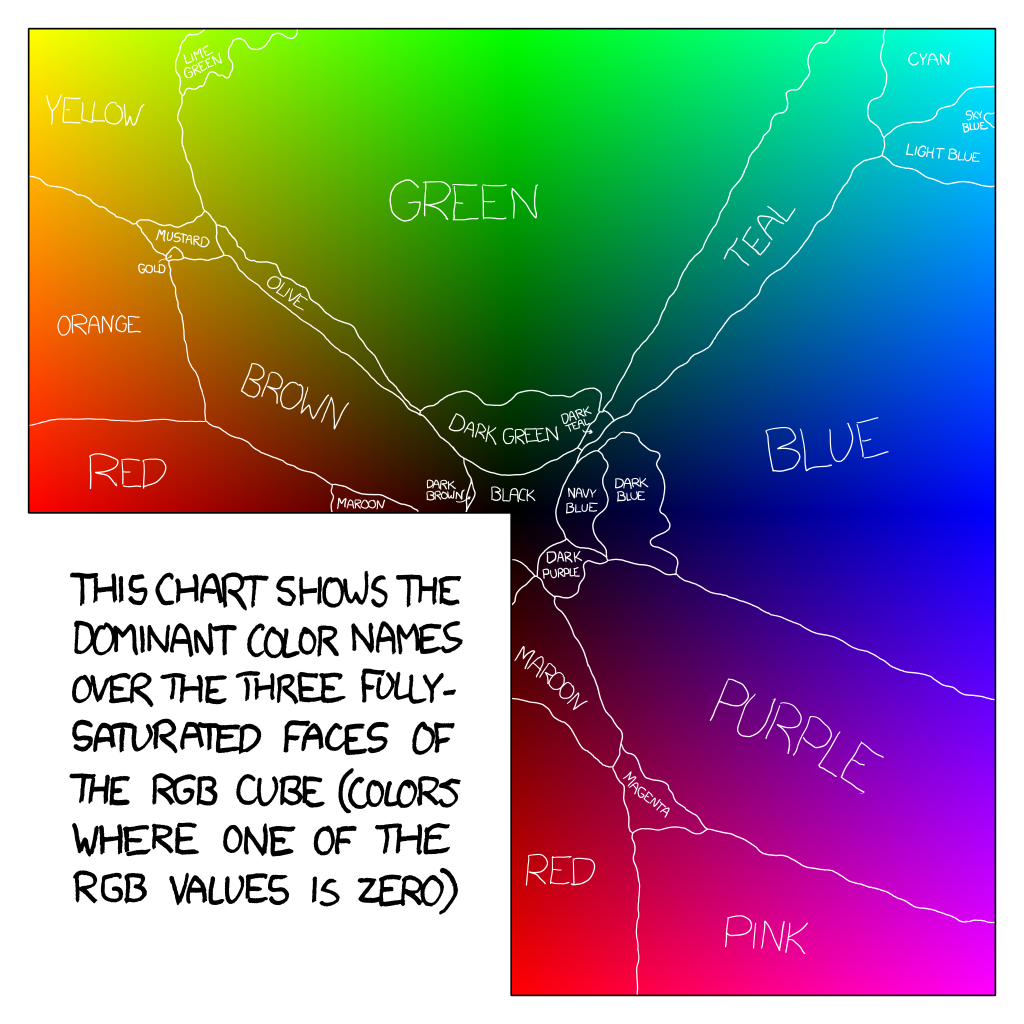
\includegraphics[width=0.5\textwidth]{images/satfaces_map.png}
  \caption[XKCD Color Survey: Color Dominant Names]{XKCD Color Survey: map of color dominant names.\protect\footnotemark{}}
  \label{fig:colornames_xkcd}
\end{figure}
%
Despite the fact XKCD's Color Survey was not a research realized with a scientific purpose, we decided to use it since it has plenty of information available to compare our results to, and it was executed with a great amount of users
which can verify it. We also found great compatibility between this survey and ours, since the values in the first were also presented in its maximum value of saturation (similar to our user study, in which we present colors in maximum hue).  \par
As said, these represent \gls{RGB} triplets but, being our user results all in accordance with the CIE XYZ Color Model, we needed some cleaning and processing to match the data our
responses. We \ul{converted the RGB to CIE XYZ values} and, then, \ul{divided all of the Color Bins in different tables}; there are 27 names atributted to colors, some have more triplets
(\emph{e.g.} blue, green or purple), but some have a smaller set, which could mean greater agreement to assign names to colors. These bins of color are represent with their frequencies, in table
\ref{table:colorbins}. \par
%
\begin{table}[htbp]
  \begin{center}
    \begin{tabular} {| c | c || c | c |}
      \hline
      Color Bin   &   Frequency   &   Color Bin   &   Frequency \\ \hline \hline
      Black       &   1782        &   Lime-Green  &   878 \\ \hline
      Blue        &   37725       &   Magenta     &   990 \\ \hline
      Brown       &   10499       &   Maroon      &   3283\\ \hline
      Cyan        &   2625        &   Mustard     &   711 \\ \hline
      Dark-Blue   &   2233        &   Navy-Blue   &   922 \\ \hline
      Dark-Brown  &   30          &   Olive       &   1336 \\ \hline
      Dark-Green  &   2927        &   Orange      &   9152 \\ \hline
      Dark-Purple &   669         &   Pink        &   12627 \\ \hline
      Dark-Red    &   2           &   Purple      &   25747 \\ \hline
      Dark-Teal   &   163         &   Red         &   15474 \\ \hline
      Gold        &   49          &   Sky-Blue    &   32 \\ \hline
      Green       &   47858       &   Teal        &   9007 \\ \hline
      Light-Blue  &   2078        &   Yellow      &   7808 \\ \hline
      Light-Green &   1           &   \-          &   \- \\
      \hline
    \end{tabular}
  \end{center}
  \caption[XKCD Color Survey: Color Bins]{XKCD Color Survey: color bins.}
  \label{table:colorbins}
\end{table}
%
The idea was to compare our answers with each color bin, to create a mapping between our users' values and commonly-used names; in order to simplify and speed up the computation
of the comparations, each color bin was drawn and the lowest polygon formed by the set of triplets of each bin was used to compare the values (instead of comparing each answer
with every triplet). Moreover, when processing these sets of RGB triplets, we left 3 color bins out of the game: \emph{Black} since it has no expressivity in the Chromaticity Diagram,
\emph{Dark-Red} and \emph{Light-Green} because they have very few triplets to be drawn. \par
%
\begin{figure}
  \centering
  \begin{minipage}{0.54\textwidth}
    \centering
    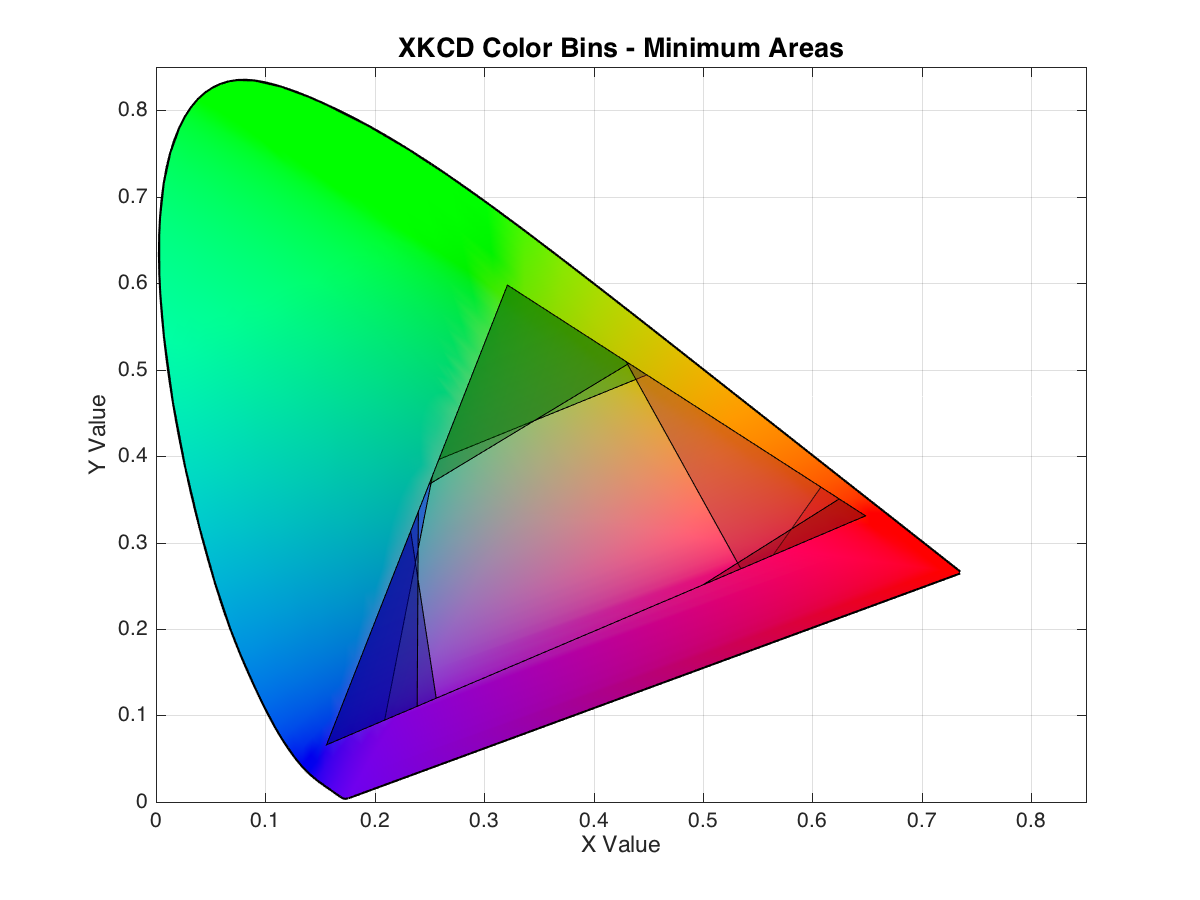
\includegraphics[width=0.9\textwidth]{images/colorbins_areas.png}
    \caption[XKCD Color Survey: Color Bins Minimum Areas]{XKCD Color Survey: Color Bins Minimum Areas.}
    \label{fig:colorbins_areas}
  \end{minipage}\hfill
  \begin{minipage}{0.45\textwidth}
    \centering
    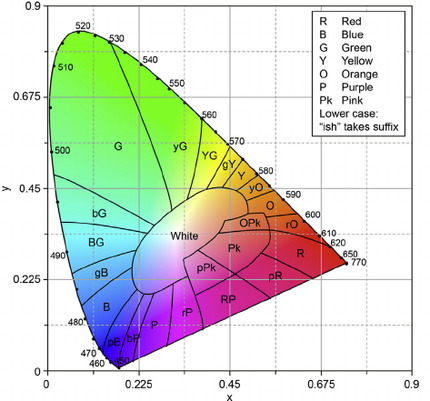
\includegraphics[width=0.87\textwidth]{images/cie_colors.png}
    \caption[Approximate Color Regions on CIE 1931 Chromaticity Diagram]{Approximate Color Regions on CIE 1931 Chromaticity Diagram. \cite{Fortner1997}}
    \label{fig:cie_colorregions}
  \end{minipage}
\end{figure}
%
However, we expected that when these color bins were drawn on a chromaticity diagram, they would create independent and more comprehensive shapes: we found that there are overlapping
values for some color bins (Figure \ref{fig:colorbins_areas}), which ultimately complicates the analysis because there is more than one possible name for the same color. For example, \emph{Blue} and \emph{Dark-Blue}
share 5 triplets: (0,0,76), (0,0,77), (0,0,78), (0,0,79) and (0,0,80); \emph{Green} and \emph{Dark-Green} share only 1 triplet, (0,57,0). No value was excluded from any color bin,
instead we solve the problem by allowing the program to find only one of the names and look no more after finding it. Moreover, the shapes created by each color bin can be depicted as \textbf{lines}
if they present contiguous values in the same edge of the triangle, or as \textbf{triangles} if the values are near the corner of the triangle and are distributed along two edges. The late situation is
represented in Figure \ref{fig:colorbins_triangle}\par
%
\begin{figure}
  \centering
  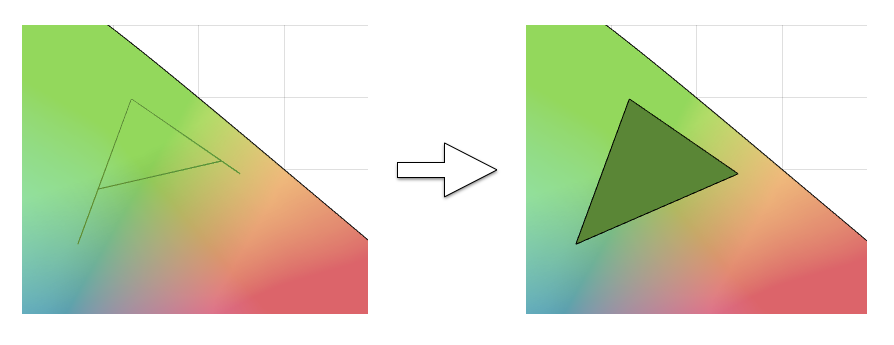
\includegraphics[width=0.8\textwidth]{images/colorbins_transformation.png}
  \caption[XKCD Color Survey: Color Bins Transformation]{XKCD Color Survey: Color Bins Transformation from line of points, to minimum polygon.}
  \label{fig:colornames_xkcd}
\end{figure} \par
%
Alternatively, we could have opted for another kind of color name detection, but its implementation would be out of the scope of this Master thesis and would take a much longer
analysis than the one performed. For instance, one could have gone for identifying the colors by analyzing their values and processing the wavelength originated, comparing the resulting
value with calculated areas, roughly defined by Brand Fortner \cite{Fortner1997} and represented on Figure \ref{fig:cie_colorregions}. This idea had one problem, which was the longevity
of its solution (dated from 1997), and the inexistence of a ready-to-go implementation, completed with an svg with all areas defined, had added weight on the decision. \par
%
Another possible method to decode color into name would be to interpret color values and associate a color temperature, being the late one compared against a well defined table
of values; the problem here was the non-existence of table of well defined values of color temperature. Further investigation is needed to ascertain the possibility of creating such
table. \par
%
\subsection{Outputs Generated}
\label{subsec:results_outputsgenerated}
%
Each script ends its execution when saving all the outputs contained in table \ref{table:outputs}: it generates a set of \gls{CSV} tables ready for being analyzed by
SPSS Program, besides creating a great amount of CIE chromaticity diagrams to support the analysis. As referred before, questions 18 to 32 do not generate any output about
white answers. \par
%
\begin{table}[htbp]
  \begin{center}
    \begin{tabular} {| c || c |}
      \hline
      Tables                    & Diagrams \\ \cline{1-2} \cline{1-2}
      age\_20\_results          & \multirow{3}{*}{\begin{tabular}[c]{@{}l@{}}For each Demographic Group:\\ - RGB, HSV and CMYK Responses \\ - CIE-L*C*h* and L*a*b* Responses \end{tabular}} \\ \cline{1-1}
      age\_20\_29\_results      &                 \\ \cline{1-1}
      age\_30\_39\_results      &                 \\ \cline{1-2}
      age\_40\_49\_results      & \multirow{4}{*}{\begin{tabular}[c]{@{}l@{}}For Laboratory Results:\\ - Regular and Daltonic Responses \\ - RGB, HSV and CMYK Responses \\ - CIE-L*C*h* and L*a*b* Responses \end{tabular}} \\ \cline{1-1}
      age\_50\_59\_results      &                 \\ \cline{1-1}
      age\_60\_results          &                 \\ \cline{1-1}
      gender\_female\_results   &                 \\ \cline{1-2}
      gender\_male\_results     & \multirow{5}{*}{\begin{tabular}[c]{@{}l@{}}For Online Results:\\ - Regular and Daltonic Responses \\ - Uncalibrated Responses \\ - RGB, HSV and CMYK Responses \\ - CIE-L*C*h* and L*a*b* Responses \end{tabular}} \\ \cline{1-1}
      gender\_other\_results    &                 \\ \cline{1-1}
      lab\_regular\_results     &                 \\ \cline{1-1}
      lab\_daltonic\_results    &                 \\ \cline{1-1}
      online\_regular\_results  &                 \\ \cline{1-2}
      online\_daltonic\_results & \multirow{3}{*}{\begin{tabular}[c]{@{}l@{}}For White Answers:\\ - White Responses \\ \end{tabular}} \\ \cline{1-1}
      online\_uncalibrated\_results &           \\ \cline{1-1}
      white\_answers            &               \\ \cline{1-2}
    \end{tabular}
  \end{center}
  \caption[Generated Outputs of Data Processing Phase]{Generated Outputs of Data Processing Phase.}
  \label{table:outputs}
\end{table}
%%%%%%%%%%%%%%%%%%%%%%%%%%%%%%%%%%%%%%%%%%%%%%%%%%%%%%%%%%%%%%%%%%%%%%%%%%%%%%%%%%%%%%%%%%%%%%%%%%%%%%%%%%%%%%%%%%%%%%%%%%%%%%%%%%%%%%%%%%%%%%%%%%%
%                                                                   RESULTS                                                                       %
%%%%%%%%%%%%%%%%%%%%%%%%%%%%%%%%%%%%%%%%%%%%%%%%%%%%%%%%%%%%%%%%%%%%%%%%%%%%%%%%%%%%%%%%%%%%%%%%%%%%%%%%%%%%%%%%%%%%%%%%%%%%%%%%%%%%%%%%%%%%%%%%%%%
\section{Results}
\label{sec:results_results}
%
In the following section, we perform a statistical analysis of the processed data obtained from the user study. The main data to be analyzed is the one obtained in the
laboratory environment, being the online data only the corroboration of the main data. We start by drawing a profile of users who responded the survey, characterizing them as the age,
country of residence, academic degree, along with other characteristics; after, we begin mapping answers to the questions raised in the beginning of study, also referred in section
\ref{sec:impl_objectives}, which comprises topics about \emph{Color Mixtures}, \emph{Color Models}, \emph{Color Naming} and consider differences between \emph{demographic groups}. \par
%
By the end of this chapter, we are going to discuss the results of the analysis and consider eventual implications for \gls{InfoVis} field of research. The following table \ref{table:summarize_results}
summarizes how the study is characterized: how many responses were given \emph{per} question, from which environment they came and the user sample from each demographic group. \par
%
\textbf{INCLUIR TABELA COM CONTAGEM.}
%
\subsection{User Profile}
\label{subsec:results_userprofile}
%
As previosuly said on section \ref{sec:results_datacleaning}, we gathered a total amount of 259 users with, at least, one valid answer: from the laboratory environment
we collected 28 users, and 231 from the online strand. All of these users gave valid answers along the Profiling, Calibration and Color Deficiencies Tests Phases: the information collected
in the Profiling page is the most important to compose a user profile. \par
Recalling section \ref{subsec:design_profiling}, we stablished that the most important informations to collect were the \emph{age}, the \emph{gender}, \emph{academic degree},
\emph{nationality} and \emph{country of residence}, as well as the \emph{native language} of each user. The table \ref{table:profiling_genderacademic} represents the frequencies of genders, ages and
academic degrees. \par
%
\begin{table}[htbp]
  \resizebox{\textwidth}{!} {
    \begin{tabular}{| l || c || c | c | c | c | c | c || c | c | c || c | c | c | c | c | c |}
      \hline
      \multicolumn{1}{|c||}{\multirow{2}{*}{Environment}} & \multirow{2}{*}{Users} & \multicolumn{6}{c||}{Ages}                                                           & \multicolumn{3}{c||}{Gender} & \multicolumn{6}{c|}{Academic Degree}                          \\ \cline{3-17}
      \multicolumn{1}{|c||}{}                             &                        & {[}0; 20{[} & {[}20; 29{]} & {[}30;39{]} & {[}40;49{]} & {[}50;59{]} & {[}60;90{]} & Female   & Male   & Other   & College & High-School & Bachelor & Master & Doctor & NoDegree \\ \hline
      Laboratory                                         & 28                     & 0           & 17           & 5           & 3           & 1           & 2            & 10       & 18     & 0        & 0       & 5           & 13       & 10     & 0      & 0        \\ \hline
      Online                                             & 231                    & 38          & 145          & 15          & 16          & 11          & 6            & 95       & 134    & 2        & 38      & 42          & 79       & 64     & 5      & 3        \\ \hline \hline
      Total                                              & 259                    & 38          & 162          & 20          & 19          & 12          & 8            & 105      & 152    & 2        & 38      & 47          & 92       & 74     & 5      & 3        \\ \hline
    \end{tabular}}
  \caption[Results: Profiling Information (Gender and Academic)]{Results: Profiling Information (Gender and Academic)}
  \label{table:profiling_genderacademic}
\end{table}
%
As seen above, our user sample is composed by 259 (100\%) users, being \textbf{105 (40.5\%) Females}, \textbf{152 (58.7\%) Males} and a minority of \textbf{2 (0.8\%) Other gendered users}: this sample age can
be characterized as being generally young ($\mu =$ 29.77, $\overline{X_{Age}} =$ 23, $\sigma =$ 40.30), surprinsigly having \textbf{8 users (3.09\%) aged above 60 years old} which could enhance some interesting
differences between age groups. Generally, our users have hight academic qualifications, representing \textbf{66.02\% of all users (Bachelor, Master and Doctoral Degrees)}, being \textbf{38 (14.67\%) users
qualified with College degree}, \textbf{47 (18.15\%) have a High-School degree} and only \textbf{3 (1.16\%) subjects do not presented any academic degree}. Between the laboratory and online environment, the distribution
of users remains with the same proportions: more male users than females, mostly aged between 20 and 29 years old (60.71\%) and the majority having a superior academic degree (46.43\% BSc and 35.71\% MSc). \par
%
\begin{table}[htbp]
  \resizebox{\textwidth}{!} {
  \begin{tabular}{| l || c || c | c | c | c | c | c || c | c | c | c | c | c || c | c | c |}
    \hline
    \multicolumn{1}{|c||}{\multirow{2}{*}{Environment}} & \multirow{2}{*}{Users} & \multicolumn{6}{c||}{Nacionality} & \multicolumn{6}{c||}{Country of Residence} & \multicolumn{3}{c|}{Languages} \\ \cline{3-17}
    \multicolumn{1}{|c||}{}                             &                        & CA  & ES & PT & UK & US & Others & CA   & DE   & GB   & PT   & US  & Others  & PT      & EN      & Others     \\ \hline
    Laboratory                                         & 28                     & 0   & 0  & 27 & 1  & 0  & 0      & 0    & 0    & 0    & 28   & 0   & 0       & 28      & 0       & 0          \\ \hline
    Online                                             & 231                    & 5   & 3  & 188& 6  & 11 & 18     & 5    & 3    & 9    & 189  & 11  & 14      & 188     & 29      & 14         \\ \hline \hline
    Total                                              & 259                    & 5   & 3  & 215& 7  & 11 & 18     & 5    & 3    & 9    & 217  & 11  & 14      & 216     & 29      & 14         \\ \hline
  \end{tabular}}
  \caption[Results: Profiling Information (Nationalities, Countries of Residence and Languages)]{Results: Profiling Information (Nationalities, Countries of Residence and Languages)}
  \label{table:profiling_nacionalities}
\end{table}
%
The table \ref{table:profiling_nacionalities} depicts nationalities, current countries of residence and native languages spoken by our users. From the 259 (100\%) participant users,
\textbf{215 (83.01\%) of them have Portuguese nationality}, \textbf{217 (83.78\%) live in Portugal} currently and \textbf{216 (83.40\%) speak Portuguese}; the second most influent group of users are from english-speaking
countries (United Kingdom, United States of America, and others). Other minor users which contributed to our survey came from Turkey, France, New Zealand, Sweden or even Antarctica (among others) -
\textbf{these countries represent only 5.41\%}. An ideal distribution of users would be such that it included enough users from all continents, which would give us room to investigate better the cultural
implications on the results; another interesting aspect would be to have the users of non-industrialized countries included in the sample, which was not accomplished in this study since an isolated vietnamese
user (0.39\% of the user sample) contributed to the study.
%
\subsection{Color Models}
\label{subsec:results_colormodels}
%
In this subsection, we analyze the results and give answers to color models' related questions, set on section \ref{sec:impl_objectives}. Along with the statistics we are going to present, we will map them against the those
questions, clearly identifying them whenever they are answered. We would like to emphasize that the important results are the ones collected in the laboratory environment: the online results will bridge and support the conclusions
extracted from the laboratory conditions. \par
%
\begin{table}[htbp]
  \resizebox{\textwidth}{!} {
  \begin{tabular}{| c | c | c | c | c | c || c | c | c | c | c | c |}
    \hline
    ID & HSV  & CIE-L*C*h* & CMYK & RGB  & CIE-L*a*b* & \multicolumn{1}{l|}{ID} & \multicolumn{1}{l|}{HSV}  & \multicolumn{1}{l|}{CIE-L*C*h} & \multicolumn{1}{l|}{CMYK} & \multicolumn{1}{l|}{RGB}  & CIE-L*a*b* \\ \hline \hline
    1  & 0.06 & 0.17       & 0.06 & 0.08 & 0.09       & \multicolumn{1}{l|}{10} & \multicolumn{1}{l|}{0.23} & \multicolumn{1}{l|}{0.25}      & \multicolumn{1}{l|}{0.01} & \multicolumn{1}{l|}{0.03} & 0.05       \\ \hline
    2  & 0.09 & 0.13       & 0.06 & 0.09 & 0.09       & \multicolumn{1}{l|}{11} & \multicolumn{1}{l|}{0.03} & \multicolumn{1}{l|}{0.13}      & \multicolumn{1}{l|}{0.13} & \multicolumn{1}{l|}{0.27} & 0.13       \\ \hline
    3  & 0.04 & 0.22       & 0.04 & 0.06 & 0.07       & \multicolumn{1}{l|}{12} & \multicolumn{1}{l|}{0.05} & \multicolumn{1}{l|}{0.23}      & \multicolumn{1}{l|}{0.12} & \multicolumn{1}{l|}{0.14} & 0.16       \\ \hline
    4  & 0.07 & 0.18       & 0.19 & 0.24 & 0.18       & \multicolumn{1}{l|}{13} & \multicolumn{1}{l|}{0.17} & \multicolumn{1}{l|}{0.14}      & \multicolumn{1}{l|}{0.18} & \multicolumn{1}{l|}{0.18} & 0.12       \\ \hline
    5  & 0.09 & 0.22       & 0.12 & 0.1  & 0.1        & \multicolumn{1}{l|}{14} & \multicolumn{1}{l|}{0.1}  & \multicolumn{1}{l|}{0.27}      & \multicolumn{1}{l|}{0.06} & \multicolumn{1}{l|}{0.13} & 0.09       \\ \hline
    6  & 0.05 & 0.1        & 0.05 & 0.07 & 0.04       & \multicolumn{1}{l|}{15} & \multicolumn{1}{l|}{0.06} & \multicolumn{1}{l|}{0.3}       & \multicolumn{1}{l|}{0.5}  & \multicolumn{1}{l|}{0.09} & 0.11       \\ \hline
    7  & 0.15 & 0.18       & 0.05 & 0.03 & 0.04       & \multicolumn{1}{l|}{16} & \multicolumn{1}{l|}{0.1}  & \multicolumn{1}{l|}{0.2}       & \multicolumn{1}{l|}{0.07} & \multicolumn{1}{l|}{0.08} & 0.04       \\ \hline
    8  & 0.08 & 0.15       & 0.03 & 0.02 & 0.05       & \multicolumn{1}{l|}{17} & \multicolumn{1}{l|}{0.05} & \multicolumn{1}{l|}{0.16}      & \multicolumn{1}{l|}{0.03} & \multicolumn{1}{l|}{0.08} & 0.07       \\ \hline
    9  & 0.05 & 0.15       & 0.09 & 0.09 & 0.1        &                         &                           &                                &                           &                           &            \\ \hline
  \end{tabular}}
  \caption[Laboratory Results: Centroids of Results Mixed in each Color Model]{Laboratory Results: Centroids of Results Mixed in each Color Model, for each question.}
  \label{table:colormodels_centroids}
\end{table}
%
As referred before, each answer pair given from our users on questions 1 to 17 (type \emph{objTwoColors}) was blendend in 5 color models: HSV, CIE-L*C*h*, CMYK, RGB and CIE-L*a*b*. Then, the XY coordinates of each resulting
mixture were mapped on a CIE Chromaticity Diagram, the centroids of each group of mixtures was calculated, and the distance from each centroid to the (ideal) pre-calculated answer was measured. The table \ref{table:colormodels_centroids}
represents the distance measured associated to each color model, for every laboratory result. \par
%
Considering an alpha of 0.05 when running the \emph{Kolmogorov-Smirnov} and \emph{Shapiro-Wilk} Normality Tests, both CIE-L*C*h* ($sig_{ks} =$ 0.200, $sig_{sw} =$ 0.430) and CIE-L*a*b* ($sig_{ks} =$ 0.200, $sig_{sw} =$ 0.221) present a
normal distribution. Analyzing the responses for each color model, the one which presented the lowest distances was the CMYK Color Model ($\tilde{x}_{CMYK} = $ 0.06), followed by HSV ($\tilde{x}_{HSV} = $ 0.07), RGB and CIE-L*a*b* with the
same values ($\tilde{x}_{RGB} = $ 0.09 and $\mu_{Lab} = $ 0.09), being CIE-L*C*h the model which has the highest calculated distances ($\mu_{LCh} = $ 0.1812). However, the color model which has the highest variance of answers is the
CMYK ($\sigma^2_{CMYK} = $ 0.013), opposed to the CIE-L*a*b* ($\sigma^2_{Lab} = $ 0.002): this may mean that, aside from having indicated closer mixtures to the desired one, users scattered more their answers when compared to the late color model. \par
%
Breaking down the results according to Color Models \emph{per} question, we obtain the following results: \par
%
\begin{itemize}
  \item \textbf{HSV Color Model Blendings} - The questions which have shorter distances are (in this order) number 11 (\textbf{0.03}), 3 (\textbf{0.04}), 6, 9, and 17 (all with \textbf{0.05}) and, lastly, question 15 (\textbf{0.06}): the majority
  of the cited questions presented a \ul{green color} and asked the user to indicate with colors did generate that particular shade. In the opposite strand, the questions with larger distances are (in this order) number 10 (\textbf{0.23}),
  13 (\textbf{0.17}), 7 (\textbf{0.15}), 14 and 16 (both \textbf{0.1}), 2 and 5 (both \textbf{0.09}): interestingly, all these questions have colors in \ul{different shades of blue or purple}, which could relate to the lacking human capability
  of accurately distinguish differentes tones of blue.
  \item \textbf{CIE-L*C*h Color Model Blendings} - The questions which have best results are number 6 (\textbf{0.1}), 5 (\textbf{0.12}), 2 and 11 (\textbf{0.13}), 13 (\textbf{0.14}), 8 and 9 (\textbf{0.15}); contrary, question 15, question 14,
  question 10, question 12 and question 3 have the lowest scores. Curiously, the best results from this color model are from questions which present \ul{red, pink and derived colors like orange}, while the weakest results came from a mix of
  questions which present green shades and blue derived ones, similar to HSV.
  \item \textbf{CMYK Color Model Blendings} - As we are about to express, the CMYK is one the color model which gathers the broadest type of results: while in some of the previous color models, the best and worst answers are concentrated on
  specific ranges of colors, the results for this model are spread across the main primitives yellow, magenta and green, red, blue shades and purples. The shorter distances are on questions 1, 8, 17, 3, 6, 7, 1, and 2, while the longer are on questions 15, 4, 13, 11, 12 and 5.
  \item \textbf{RGB Color Model Blendings} - Results from RGB centroids are quite similar to CMYK results, which is no surprise since they are relatively similar opposite models and explained on the theorical background of this document.
  The shorter distances are on questions 8, 7, 10, 6, 3, 1, 16 and 17 while the longer are on questions 11, 4, 13, 11, 12 and 14.
  \item \textbf{CIE L*a*b* Color Model Blendings} - This color model is the one, by far, which builds more consensus, since there are much more questions which present the smallest number of weak (longer) distances to the ideal answer pair.
  The shorter distances questions are on questions 6, 7, 16 (all with \textbf{0.04}), 8 and 10 (both \textbf{0.05}), 3 (\textbf{0.07}), 1, 2 and 14 (all with \textbf{0.09}) and, finally, 5 and 9 (\textbf{0.1}); while the longer are on questions
  4, 12, 11, 13 and 15.
\end{itemize}
%
incluir diagramas! \\
falar de questões que originaram mais frequentemente melhores resultados e piores, para extrair as cores dos mesmos. \par
abordar questão de que modelos originaram melhores respostas, se são aditivos ou subtrativos. \\
verificar adicionalmente para o modelo HSV, qual a disposição das cores no circulo de cores. \\
fazer analise concreta das questões 1, 2, 7, 8 e 17, que são as primitivas. perceber se resultados são positivos para a geração de primitivas com base noutras. \\
tentar fazer uma análise dos resultados, para perceber se há muita discretização. \\
%
\subsection{Color Mixtures}
\label{subsec:results_colormixtures}
%
Regarding the color mixtures' related questions, we would like to make the following analysis. We asked at \ref{sec:impl_objectives} ... \par
%
Fazer também mistura mais fácil, comparando os ratings das questões e ver qual a mistura que apresenta melhores resultados. \\
Comparar misturas que originam a mesma cor, com base em primárias diferentes e perceber se utilizadores conseguem detectar várias
misturas para uma mesma cor.
%
\subsection{Color Naming}
\label{subsec:results_namingcolors}
%
Cores mais comuns em algumas perguntas; existe alguma ordem caracteristica quando utilizador especifica uma mistura? \\
Comparar se, mais do que pelos valores anteriormente calculados, se users identificam "uma mistura de vermelho com azul" como dando um resultado
magenta, ou mais afinado para uma dada cor.
%
\subsection{Demographic Groups}
\label{subsec:results_demographic}
%
Fazer apenas comparação de faixas etárias entre si, e géneros entre si. \\
Uma ánalise interesse seria comparar faxias etárias por género, mas seria necessária uma amostra bastante mais significativa para cada grupo.
%
%%%%%%%%%%%%%%%%%%%%%%%%%%%%%%%%%%%%%%%%%%%%%%%%%%%%%%%%%%%%%%%%%%%%%%%%%%%%%%%%%%%%%%%%%%%%%%%%%%%%%%%%%%%%%%%%%%%%%%%%%%%%%%%%%%%%%%%%%%%%%%%%%%%
%                                                                DISCUSSION                                                                       %
%%%%%%%%%%%%%%%%%%%%%%%%%%%%%%%%%%%%%%%%%%%%%%%%%%%%%%%%%%%%%%%%%%%%%%%%%%%%%%%%%%%%%%%%%%%%%%%%%%%%%%%%%%%%%%%%%%%%%%%%%%%%%%%%%%%%%%%%%%%%%%%%%%%
%
\section{Discussion}
\label{sec:results_discussion}
%
Fazer apanhado dos resultados todos. \par
%
\subsection{Calibration Resiliency}
\label{subsec:results_calibration}
%
Como verificamos ainda alguns users com calibração imprópria para teste, considerámos que poderia ser uma fonte de resultados
interessantes. Como tal, criámos um dataset para os mesmos e comparámos com os resultados dos utilizadores calibrados. Os resultados
são os que se seguem... \par
%
\subsection{Creation of Color Scales}
\label{subsec:results_discussion_colorscales}

\subsection{Color Organization}
\label{subsec:results_discussion_colororganization}

\subsection{Consequences for InfoVis}
\label{subsec:results_discussion_infovis}
%
Resumo dos resultados todos e regras que se podem levar deste trabalho para a área de InfoVis em geral.
%
